\documentclass[english]{SPFShortReport}
\usepackage{subfigure}
\usepackage{longtable}
\usepackage[utf8]{inputenc}
\usepackage{url}
\usepackage{adjustbox}
\usepackage{gensymb}
\usepackage{booktabs}
\usepackage[yyyymmdd,hhmmss]{datetime}
\reportName{HydD\_mfb30\_real\_dryN-CityBAS\_dryNAc1.0x58.086Vice0.4x58.086HP1.0x18.442-Year0}
\reportSubName{Energy generation costs} 
\reportDate{\today \hspace{0.1cm} at: \currenttime \hspace{0.1cm} h} 
\author{Test Author}
\address{test.author@test.com}
\begin{document}
\begin{table}[!ht]
\centering
\caption{Assumptions for calculation of heat generation costs}
\begin{adjustbox}{max width =\textwidth}
\begin{tabular}{l | c c c } 
\hline
\hline
$$ &$$ &$$ &$$ \\ 
\hline
Rate & 3.0 \% per annum\\
Analysis period & 30 years\\
Maintenance & 1.0 \% of Investment costs per year \\
\hline \\
Electricity & Fix costs:  0  Fr. per year \\
 & Variable costs:  0.20 $Fr.$ $per$ $kWh$ \\
Increase of electricity costs & 0.0 \% per year \\
Electricity costs year 1 & 4698 Fr. in year 1 \\
Energy demand per year & 57958 kWh \\
\hline
\hline
\end{tabular}
\end{adjustbox}
\label{definitionTable}
\end{table}
\begin{table}[!ht]
\centering
\caption{System and Heat generation costs (all values incl. 8$\%$ VAT) }
\begin{adjustbox}{max width =\textwidth}
\begin{tabular}{l | c c c c c } 
\hline
\hline
Group &Component &Costs &Size &LifeTime &Total Costs \\ 
 & &[CHF] & &Years &[CHF]\\ 
\hline
\\
\textbf{TES} & Storage (Stainless Steel) & -2000+10173$^{\mathrm{+250}}_{\mathrm{-100}}$/m$^3$ & 2.00 m$^3$ & 30 & 18345.6$^{\mathrm{+500.0}}_{\mathrm{-200.0}}$ (13.0$^{\mathrm{+0.4}}_{\mathrm{-0.2}}$\%) \\
 & Storage (Steel) & 666+1214/m$^3$ & 1.30 m$^3$ & 30 & 2238.2 (1.6$^{\mathrm{+0.0}}_{\mathrm{-0.0}}$\%) \\
 & electric rod & 600+0/m$^3$ & 2.00 m$^3$ & 30 & 600.0 (0.4$^{\mathrm{+0.0}}_{\mathrm{-0.0}}$\%) \\
&\cline{1-5}
 & \textbf{Total TES} & & & & 21183.8$^{\mathrm{+500.0}}_{\mathrm{-200.0}}$ (15.0$^{\mathrm{+0.4}}_{\mathrm{-0.2}}$\%) \\
\hline \\
\textbf{Col} & Collector & 9282+875/m$^2$ & 58.09 m$^2$ & 30 & 60107.2 (42.5$^{\mathrm{+0.1}}_{\mathrm{-0.1}}$\%) \\
\hline \\
\textbf{IceStorage} & Ice Storage (inc. installation) & 0+850/m$^3$ & 23.23 m$^3$ & 20 & 19749.2 (14.0$^{\mathrm{+0.0}}_{\mathrm{-0.0}}$\%) \\
\hline \\
\textbf{Hp} & HeatPump & 8194+363/kW & 18.44 kW & 20 & 14888.4 (10.5$^{\mathrm{+0.0}}_{\mathrm{-0.0}}$\%) \\
\hline \\
\textbf{Hydraulics} & Hydraulics & 11500+0/kW & 18.44 kW & 30 & 11500.0 (8.1$^{\mathrm{+0.0}}_{\mathrm{-0.0}}$\%) \\
\hline \\
\textbf{Installation system} & Installation System & 14000+0/kW & 18.44 kW & 30 & 14000.0 (9.9$^{\mathrm{+0.0}}_{\mathrm{-0.0}}$\%) \\
\hline \\
 & \textbf{Total Investment Cost} & & & & \textbf{141428.71$^{\mathrm{+500.00}}_{\mathrm{-200.00}}$} (100\%) \\ 
\hline \\ 
\hline \\ 
Annuity & Annuity (yearly costs over lifetime)  &&& & 13889$^{\mathrm{+31}}_{\mathrm{-12}}$ /a  \\
 & Share of Investment & &&& 7777$^{\mathrm{+26}}_{\mathrm{-10}}$ /a (56$^{\mathrm{+ 0}}_{\mathrm{- 0}}$\%) \\
 & Share of Electricity & 0+0.20/kWh & 23491 kWh &  & 4698 /a (34$^{\mathrm{+ 0}}_{\mathrm{- 0}}$\%)\\
 & Share of Maintenance & &&& 1414$^{\mathrm{+ 5}}_{\mathrm{- 2}}$ /a (10$^{\mathrm{+ 0}}_{\mathrm{- 0}}$\%)\\ 
 & Share of Residual Value &&& &  0 /a ( 0\%)\\
Present Value  & Present Value of all costs  & &&& 261237.88$^{\mathrm{+598.00}}_{\mathrm{-239.20}}$ CHF \\
\hline \\ 
 Energy Generation Costs & Using annuity: &&& 23.96$^{\mathrm{+0.05}}_{\mathrm{-0.02}}$ & Rp./kWh \\
\hline
\hline
\end{tabular}
\end{adjustbox}
\label{CostsTable}
\end{table}
\begin{figure}[!htbp]
\begin{center}
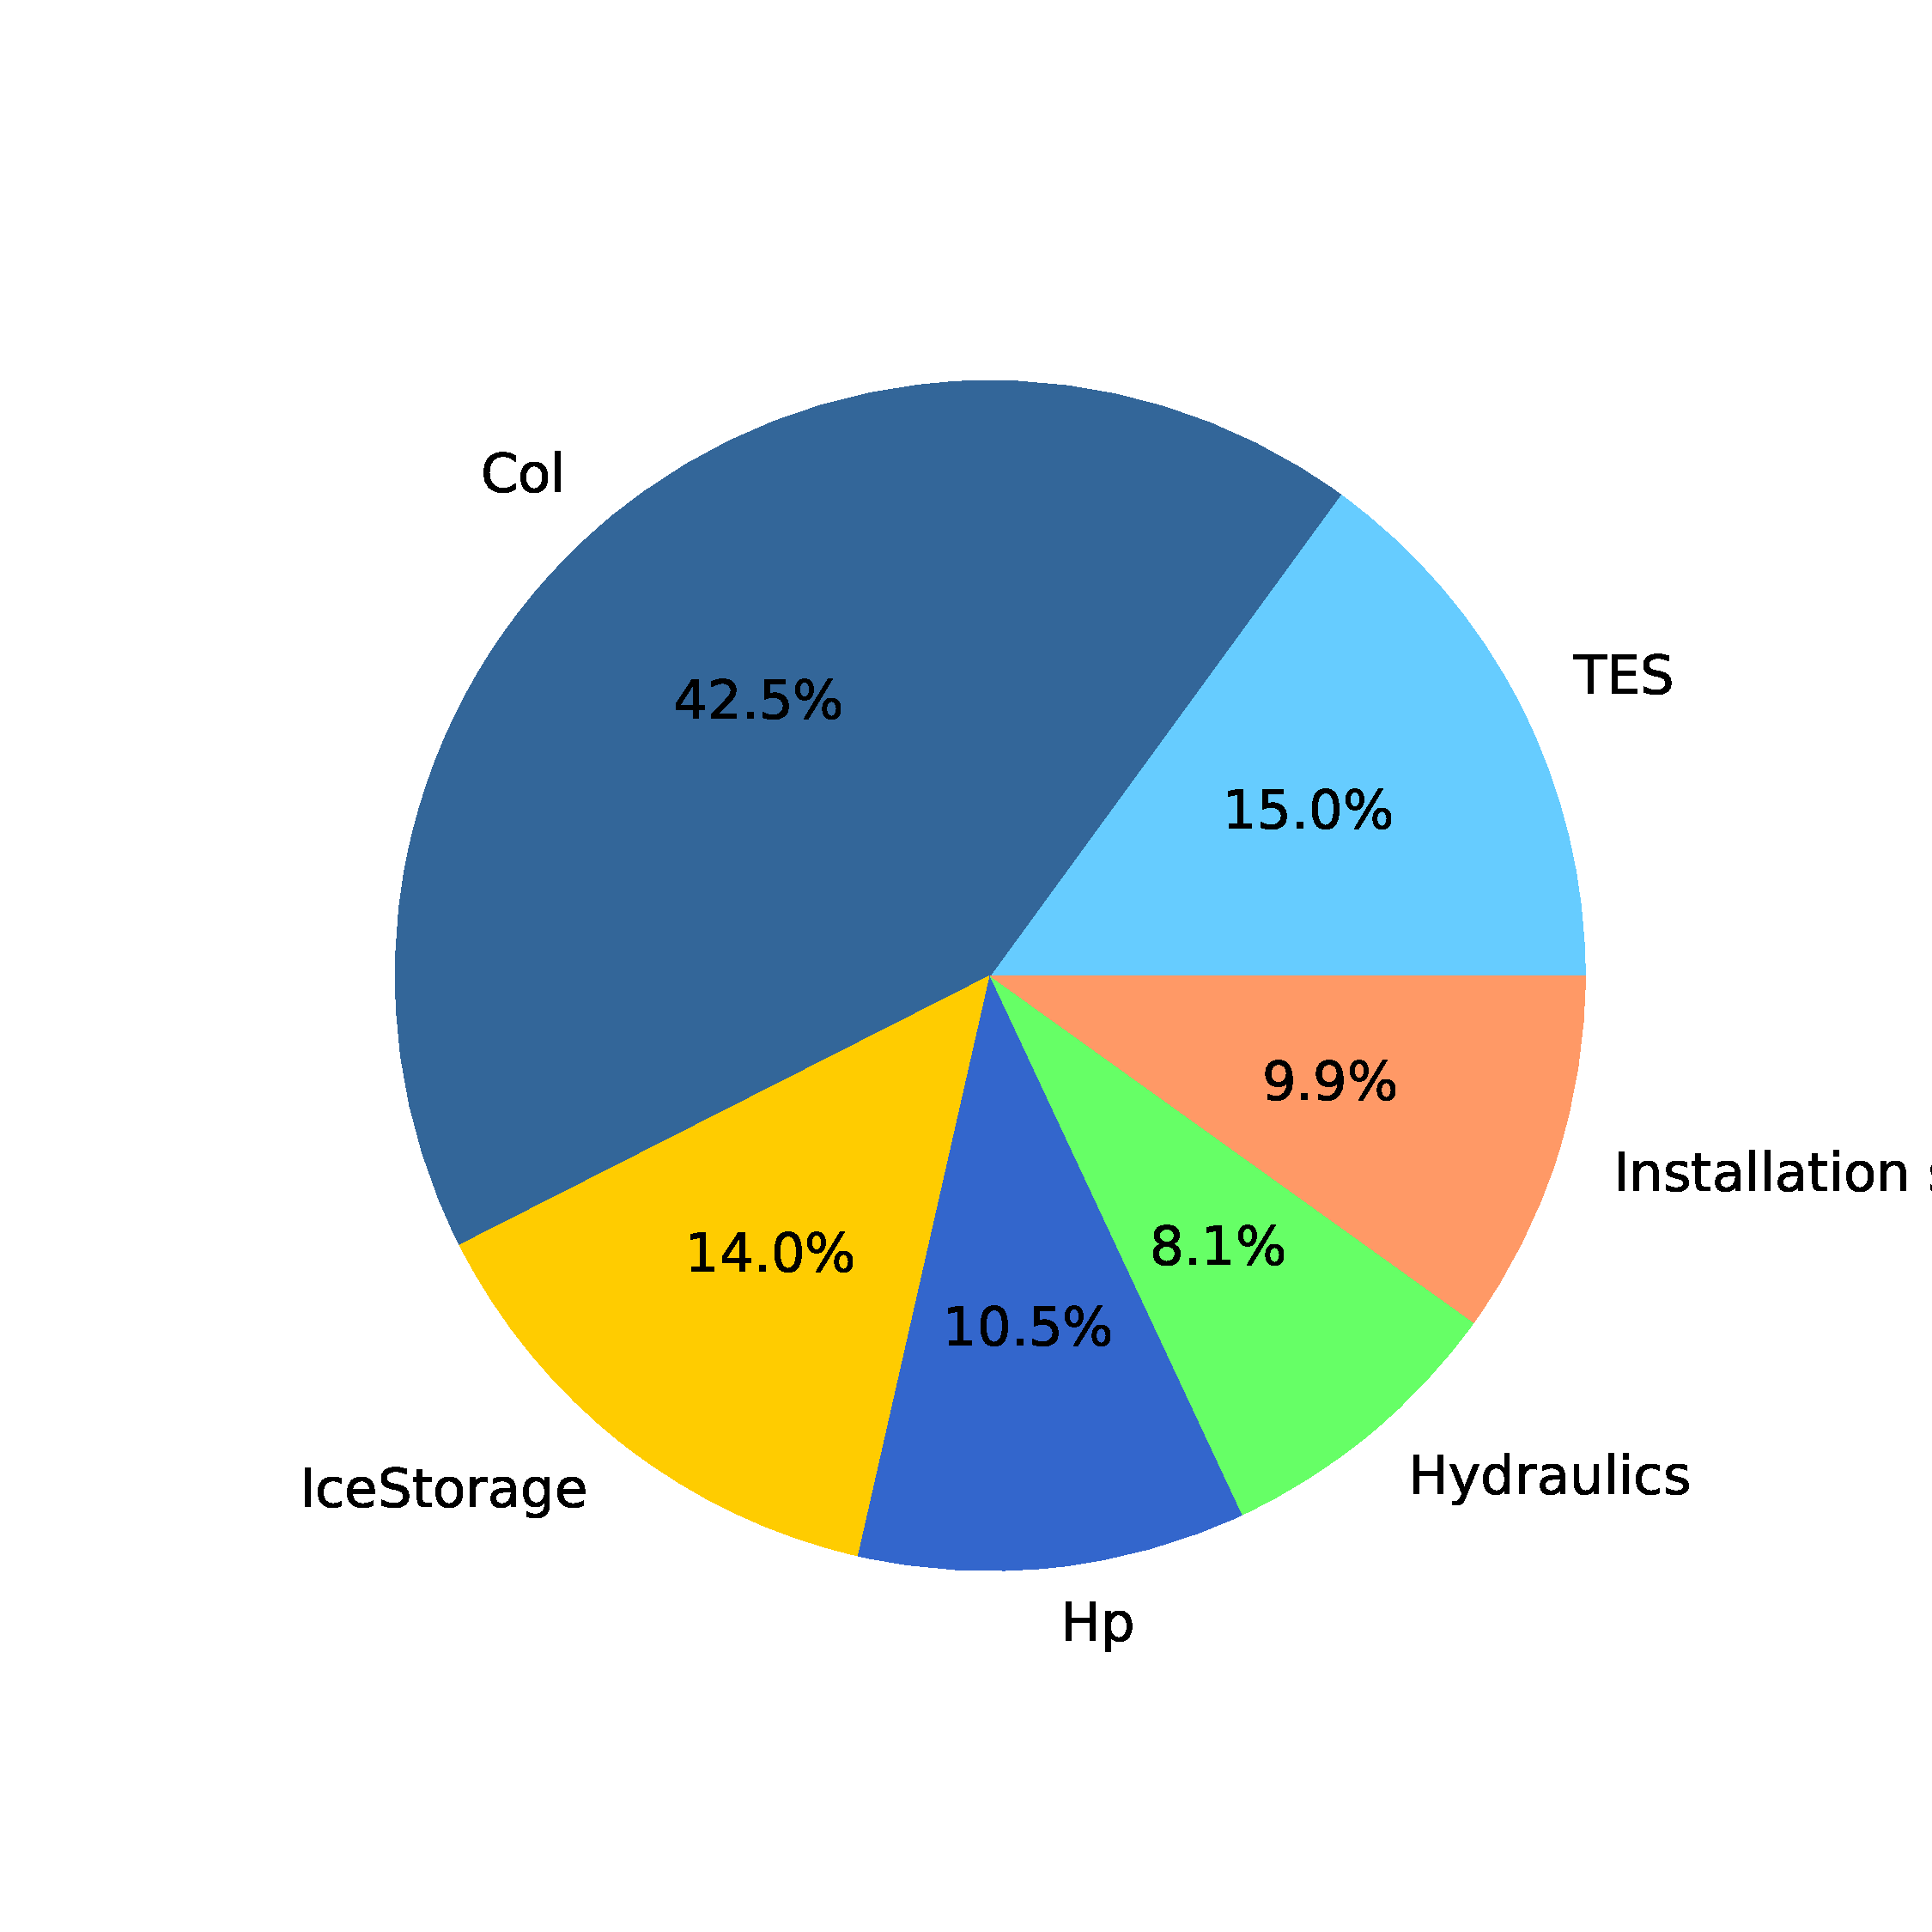
\includegraphics[width=1\textwidth]{costShare-HydD_mfb30_real_dryN-CityBAS_dryNAc1.0x58.086Vice0.4x58.086HP1.0x18.442-Year0.pdf}
\caption{System cost}
\label{systemCost}
\end{center}
\end{figure}
\begin{figure}[!htbp]
\begin{center}
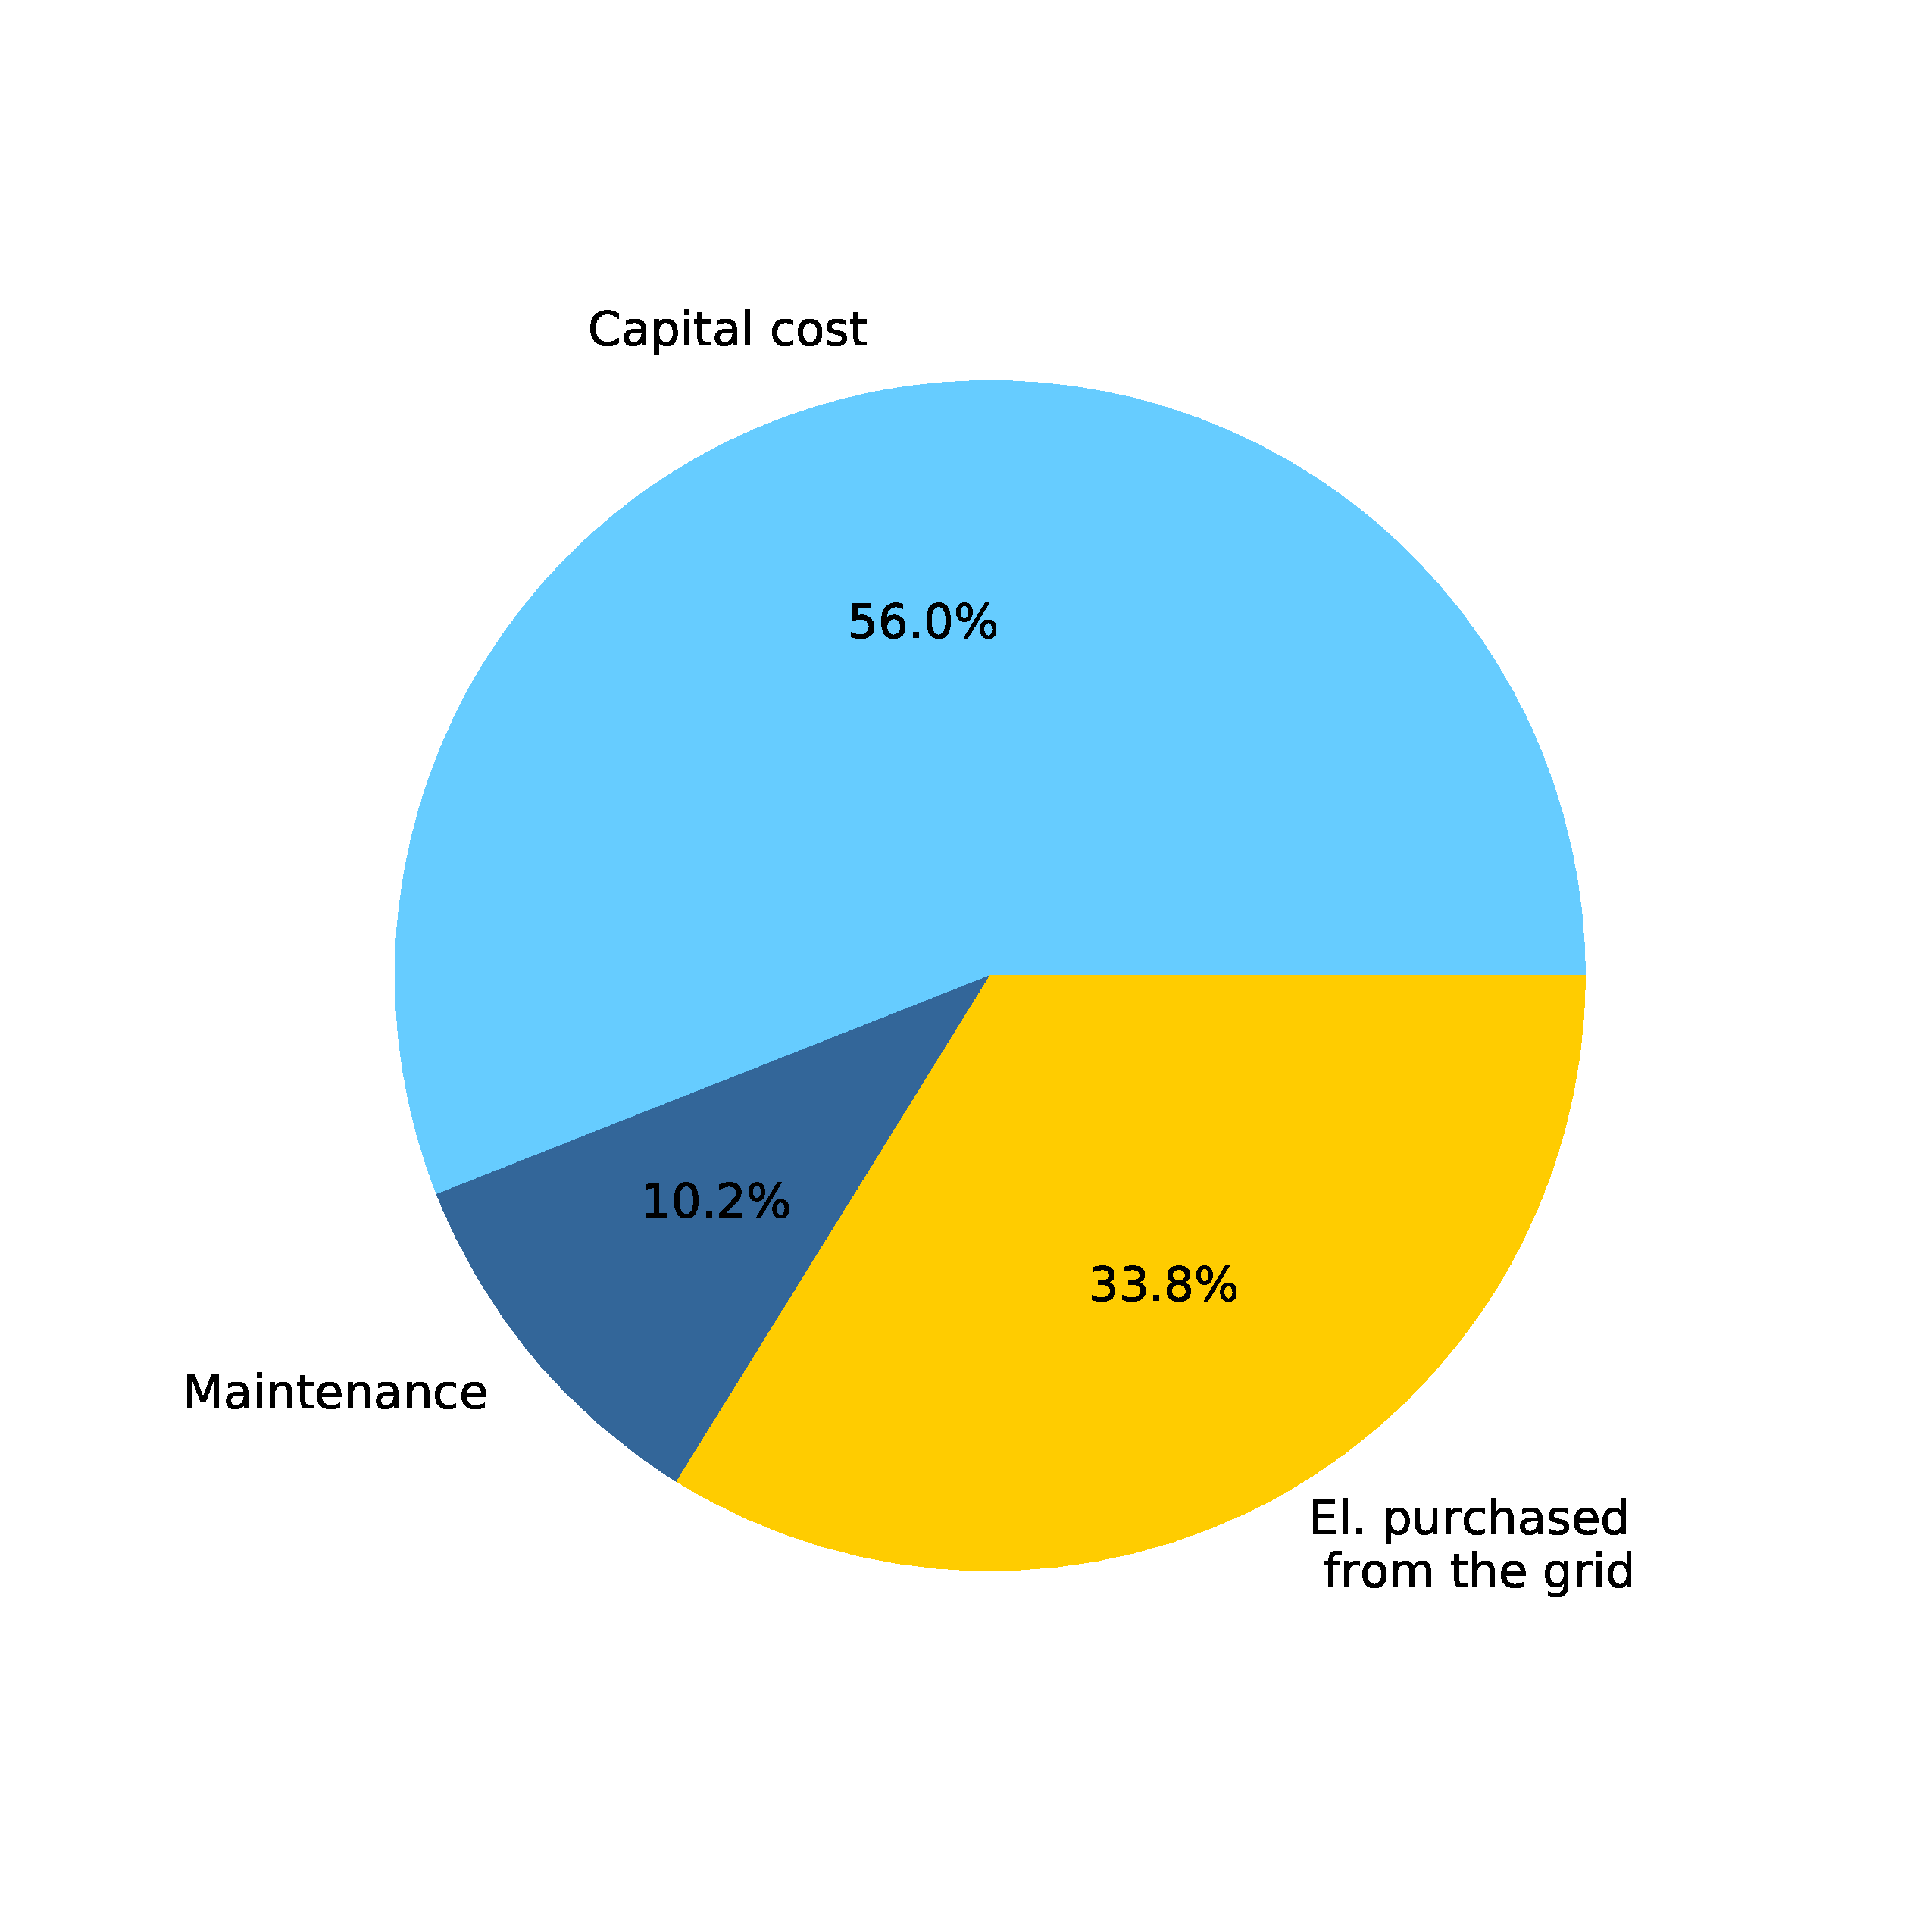
\includegraphics[width=1\textwidth]{costShareAnnuity-HydD_mfb30_real_dryN-CityBAS_dryNAc1.0x58.086Vice0.4x58.086HP1.0x18.442-Year0.pdf}
\caption{System cost annuity share}
\label{systemCostannuity}
\end{center}
\end{figure}
\end{document}
